\documentclass[12pt]{article}
\usepackage[polish]{babel}
\usepackage[utf8]{inputenc}
\usepackage[T1]{fontenc}
\usepackage{lmodern}
\usepackage{graphicx}
\usepackage{subcaption}
\usepackage{listings}
\usepackage{color}
\usepackage[svgnames]{xcolor}
\usepackage[a4paper,bindingoffset=0.2in,%
left=1in,right=1in,top=1.5in,bottom=1.5in,%
footskip=.25in]{geometry}

\definecolor{dkgreen}{rgb}{0,0.6,0}
\definecolor{gray}{rgb}{0.5,0.5,0.5}
\definecolor{mauve}{rgb}{0.58,0,0.82}

\lstset{frame=tb,
	language=Python,
	aboveskip=3mm,
	belowskip=3mm,
	showstringspaces=false,
	columns=flexible,
	basicstyle={\small\ttfamily},
	numbers=none,
	numberstyle=\tiny\color{gray},
	keywordstyle=\color{blue},
	commentstyle=\color{dkgreen},
	stringstyle=\color{mauve},
	breaklines=true,
	breakatwhitespace=true,
	tabsize=3,
	extendedchars=true,
	literate={ą}{{\k a}}1 {ę}{{\k e}}1 {ś}{{\'s}}1 {ć}{{\'c}}1 {ź}{{\'z}}1 {ż}{{\. z}}1 {ń}{{\'n}}1 {ł}{{\l}}1 {ó}{{\'o}}1,
}

\pagenumbering{gobble}
\graphicspath{{./zdjs/}}


\begin{document}
\title{Sprawozdanie - Odtwarzanie muzyki z nut na pięciolinii}
\author{Marcin Zatorski 136834, Sebastian Michoń 136770}
\date{\vspace{-2ex}}
\maketitle

\section{Cel i zakres projektu}
Celem projektu było zaimplementowanie aplikacji odczytującej nuty z obrazu z kamery, a następnie odtworzenie ich za pomocą głośnika z użyciem płytki Raspberry Pi.

\begin{figure}[h!]
	\centering
	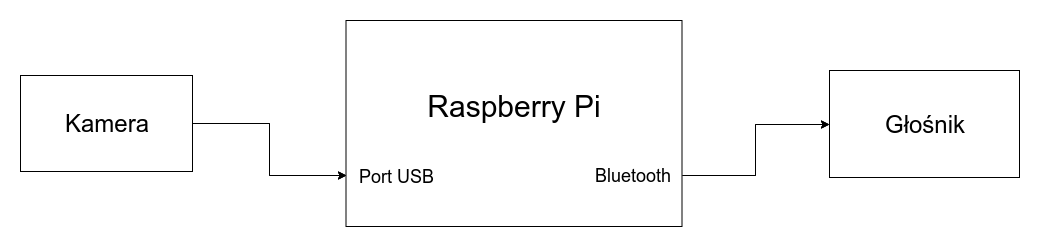
\includegraphics[width=0.9\linewidth]{SW-schematic.png}
	\caption{Schemat połączeń}
	\label{fig:schemat}
\end{figure}
	
\section{Projekt a realizacja}
Aplikacja została napisana w języku Python i Cython. Rozpoznawanie nut zostało zaimplementowane przy użyciu biblioteki OpenCV. Aplikacja jest w stanie rozpoznać nuty z wysoką skutecznością, o ile zdjęcie zostało zrobione w dobrych warunkach oświetleniowych. Algorytm rozpoznaje tylko część symboli - nuty (całe nuty, półnuty, ćwierćnuty i ósemki) oraz klucze. Tą część algorytmu można rozszerzyć o rozpoznawanie większej ilości symboli. Dokładność rozpoznawania nut również można ulepszyć na przykład poprzez zastosowanie metod uczenia maszynowego.
	
W trakcie rozwijania projektu dużą przeszkodą była szybkość działania. Dzięki przepisaniu części kodu do języka Cython oraz optymalizacjom aplikacja działa zadowalająco szybko.

Pierwotnie w projekcie zakładaliśmy użycie płytki BeagleBone Black. Zdecydowaliśmy się jednak na wykorzystanie Raspberry Pi - umożliwiło to proste podłączenie głośnika przez Bluetooth.

Do syntezy muzyki wykorzystaliśmy biblioteki mingus i fluidsynth. Dźwięk jest odtwarzany przez głośnik podłączony przez Bluetooth. Aplikacja nie pozwala na wybranie dźwięku instrumentu, co było początkowo planowane. Aplikacja nie odtwarza nut z obu pięciolinii jednocześnie - są odtwarzane po kolei.

Program można rozwinąć o lepszy interfejs użytkownika. Obecnie aplikacja jest uruchamiana z linii poleceń. Warto dodać na przykład GUI pokazujące obraz z kamery lub przycisk umożliwiający wykonanie zdjęcia. Brak interfejsu utrudnia ocenę, czy aplikacja działa poprawnie.

\section{Kluczowe fragmenty kodu}
Główna część programu, odpowiedzialna za odtwarzanie dźwięku:
\begin{lstlisting}[language=Python]
import cv2 as cv
from mingus.midi import fluidsynth

# Odczytanie obrazu z kamery
video_capture = cv.VideoCapture(0)
_, image = video_capture.read()
# Rozpoznanie nut
notes = process_image(image)
track = parse_notes(notes)
# Synteza i odtwarzanie dźwięku
fluidsynth.init(soundfont, 'alsa')
fluidsynth.play_Track(track)
\end{lstlisting}

Uproszczone funkcje odpowiedzialne za rozpoznawanie nut:
\begin{lstlisting}[language=Python]
def process_image(image):
	img, img_original, staff_lines = remove_staff_lines(image)
	notes = detect_notes(img, img_original, staff_lines)
	return notes
	
def remove_staff_lines(input_img):
	# Zmiana kolorów obrazka z odcieni szarości na czarno-biały
	imv = binarization(input_img) 
	# Rotacja obrazka tak, aby linie pięciolinii były w następnym kroku zawsze pod tym samym kątem
	img2 = rotate_image(imv, input_img)
	# Usunięcie wszystkich linii, których kąt względem dolnej krawędzi obrazka to 0
	sol = findlinez(img2) 
	# Znalezienie parametrów usuwanych wcześniej linii i połączenie ich w pięciolinie
	result = line5finder(sol, img2) 
	return img2, input_img, result
	
def detect_notes(img, img_original, staff_lines):
	templates = read_templates()
	detect_clefs(img, staff_lines) # Wykrycie kluczy: basowego i wiolinowego
	detect_noteheads(templates) # Detekcja główek nut za pomocą dopasowania wzorców
	check_if_empty(img) # Sprawdzenie czy nuta jest półnutą lub całą nutą
	detect_stems(img) # Wykrycie ogonka nuty
	check_if_eightnote(img) # Sprawdzenie czy nuta jest ósemką
\end{lstlisting}


\section{Zdjęcia urządzenia}
\begin{figure}[h!]
	\centering
	\begin{subfigure}[b]{0.32\linewidth}
		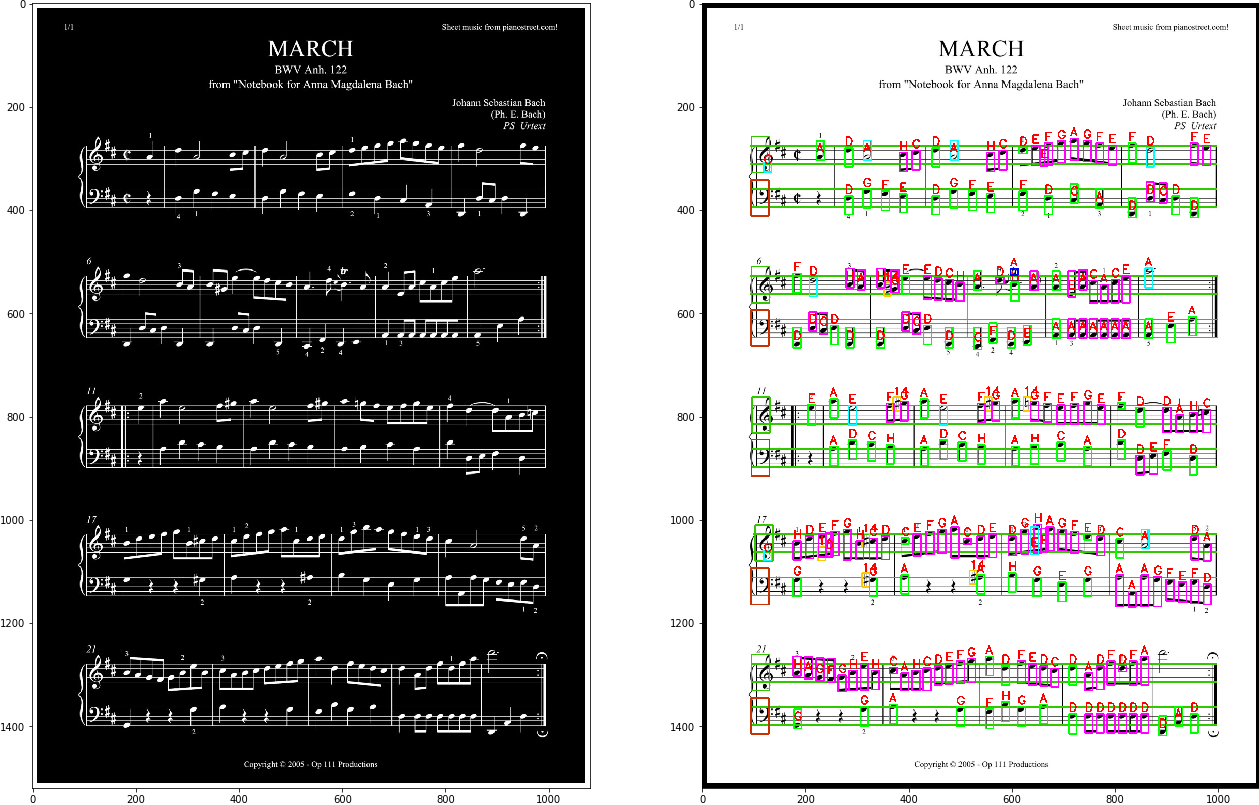
\includegraphics[width=\linewidth]{Zdj0.png}
		\caption{Pierwszy podpis}
	\end{subfigure}
	\begin{subfigure}[b]{0.32\linewidth}
		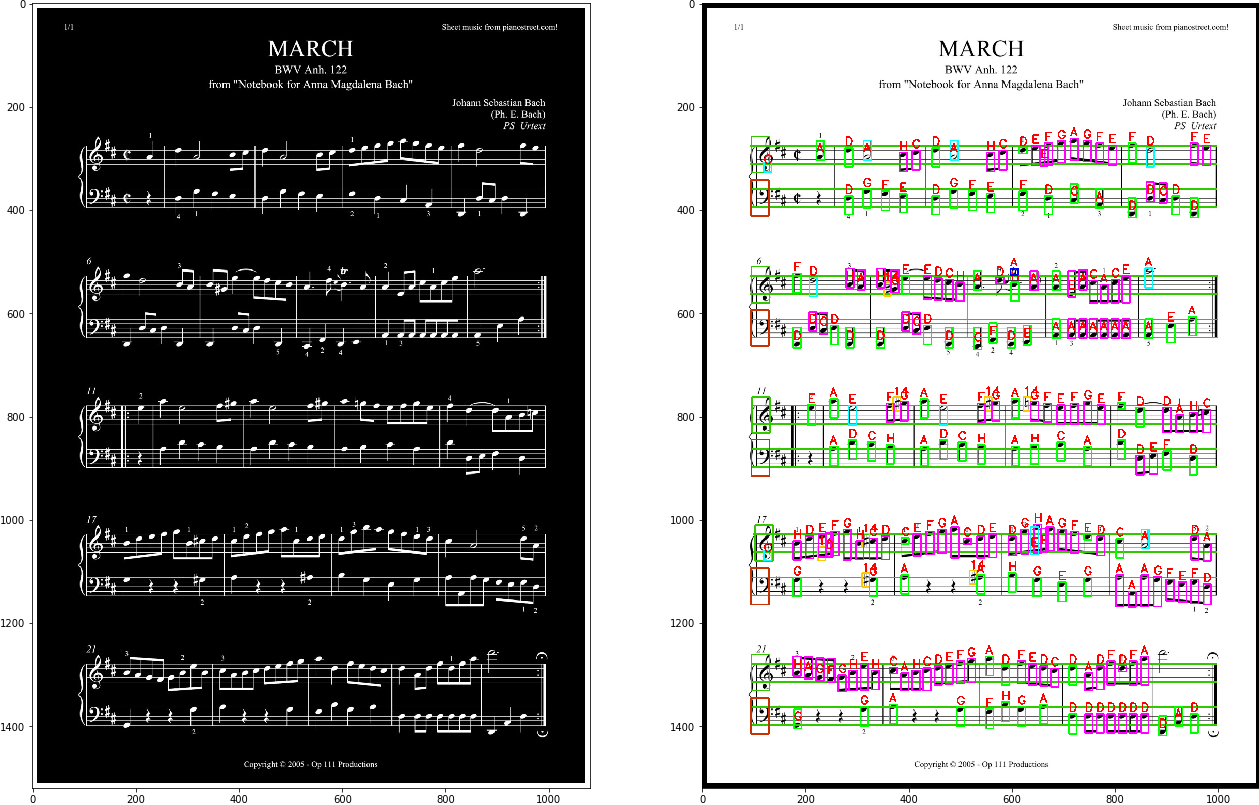
\includegraphics[width=\linewidth]{Zdj0.png}
		\caption{Drugi podpis}
	\end{subfigure}
	\begin{subfigure}[b]{0.32\linewidth}
		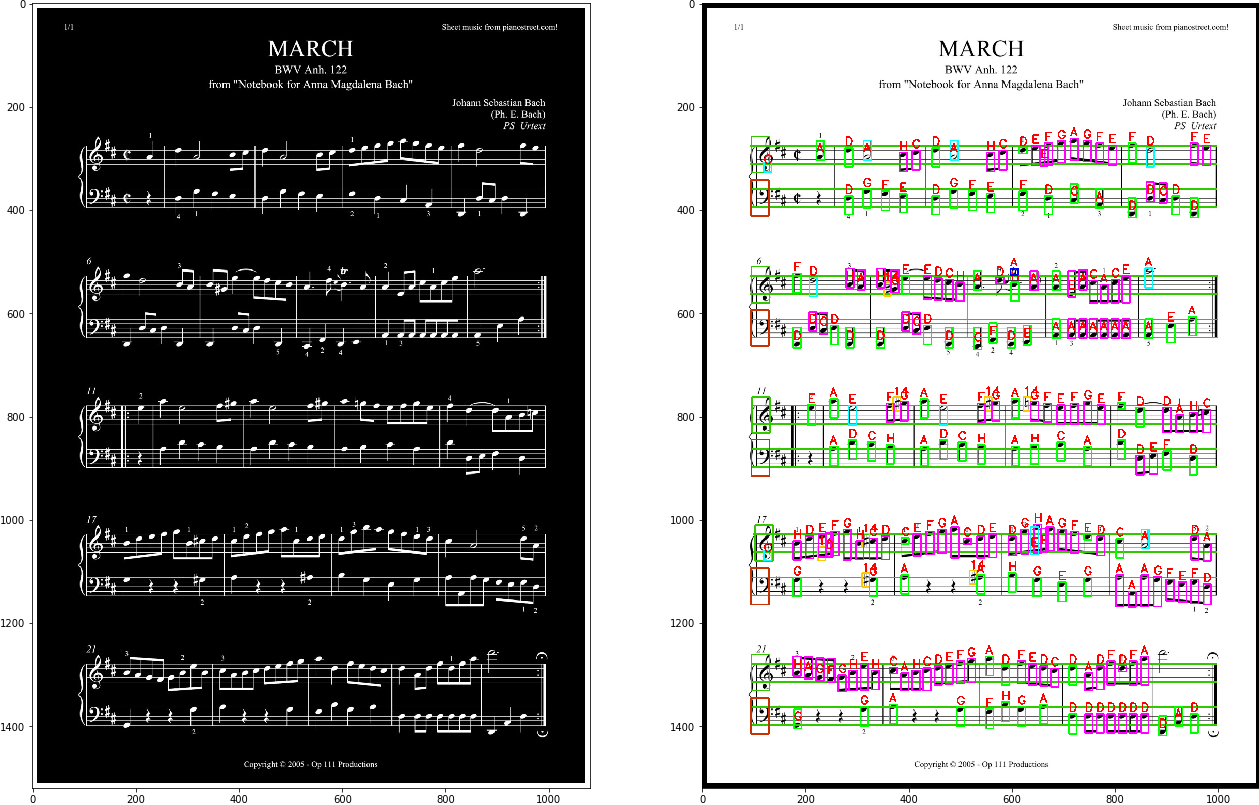
\includegraphics[width=\linewidth]{Zdj0.png}
		\caption{Trzeci podpis}
	\end{subfigure}
	
	\begin{subfigure}[b]{0.48\linewidth}
		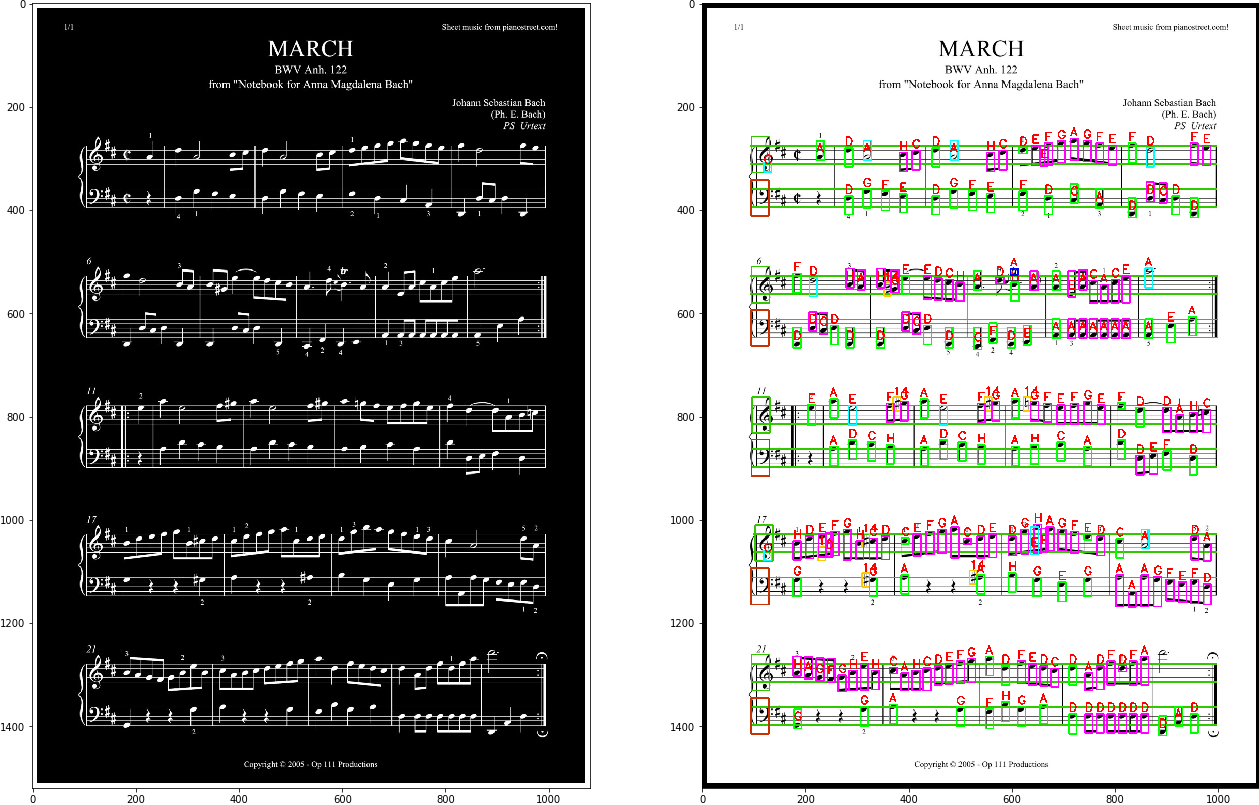
\includegraphics[width=\linewidth]{Zdj0.png}
		\caption{Czwarty podpis}
	\end{subfigure}
	\begin{subfigure}[b]{0.48\linewidth}
		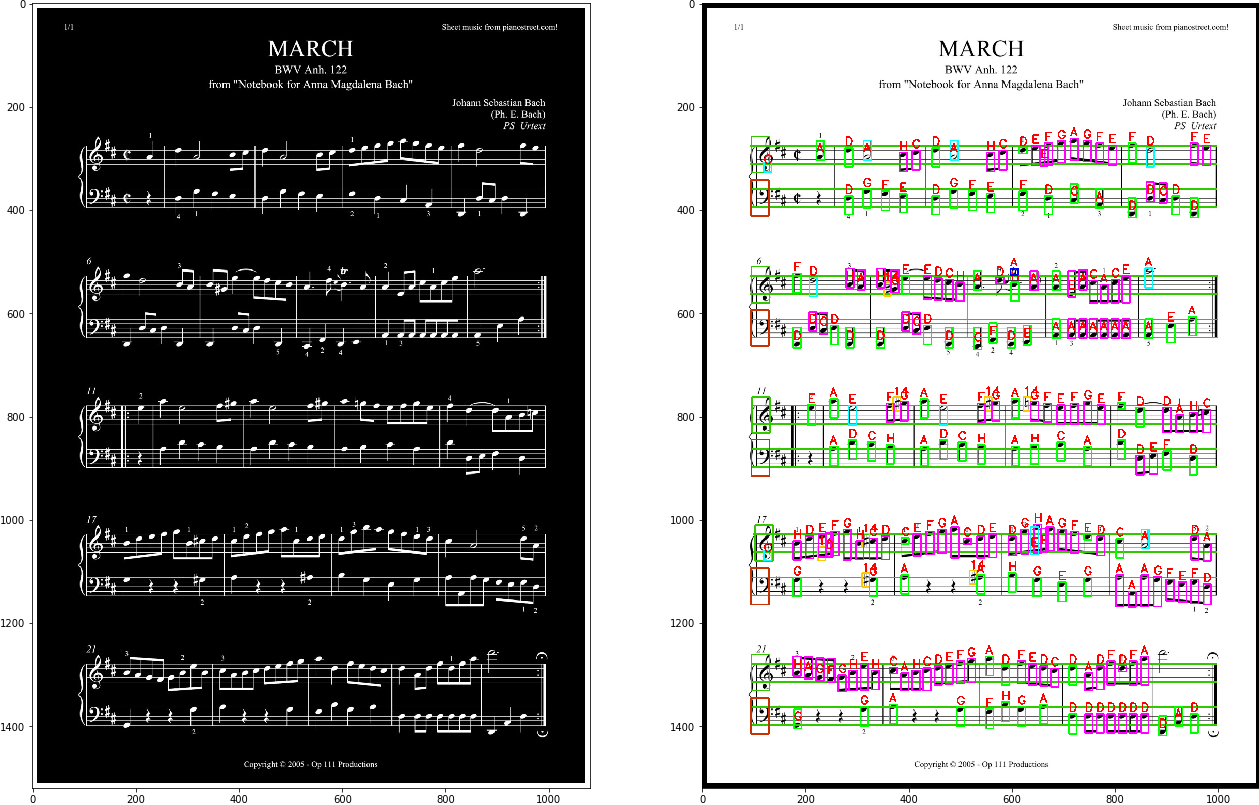
\includegraphics[width=\linewidth]{Zdj0.png}
		\caption{Piąty podpis}
	\end{subfigure}
\end{figure}

\section{Podsumowanie, wnioski}
Aplikacja realizuje swój cel, choć są elementy które można poprawić lub które nie zostały zaimplementowane. Użyty przez nas algorytm uzyskuje wysoką skuteczność przy dobrej jakości zdjęciach; zasadna byłaby próba ulepszenia kodu poprzez użycie metod adaptatywnych, opartych na funkcji kosztu zamiast metod analitycznych przetwarzania obrazu.

\end{document}
